\documentclass[11pt,a4paper]{article}

\usepackage[margin=2.5cm]{geometry}
\usepackage[T1]{fontenc}
\usepackage[utf8]{inputenc}
\usepackage{lmodern}
\usepackage{microtype}
\usepackage{amsmath,amssymb}
\usepackage{booktabs}
\usepackage{float}
\usepackage{tabularx}
\usepackage{enumitem}
\usepackage{xcolor}
\usepackage{tikz}
\usetikzlibrary{arrows.meta,positioning}
\usepackage[hidelinks]{hyperref}

\usepackage{xurl}
% Code and paths break at any character instead of overflowing the margin.
\DeclareUrlCommand\code{\urlstyle{tt}}
\newcommand{\cmd}[1]{\texttt{#1}}
\newcommand{\file}[2]{\code{#1}:#2}
\newcommand{\status}[1]{\textsf{\small #1}}
\newcommand{\pending}[1]{\textcolor{red}{[pending: #1]}}

\newenvironment{finding}[2]{%
  \subsection*{#1\texorpdfstring{\quad}{ } #2}%
  \addcontentsline{toc}{subsection}{#1\texorpdfstring{\quad}{ } #2}%
  \begin{description}[leftmargin=0pt,itemsep=3pt,font=\normalfont\bfseries]%
}{\end{description}}

\title{Security analysis of the C2PA location attestation pipeline}
\author{Patricio Peralta Ramos \and Martina Monastra \and Luz Alba Posse\\[2pt]
  \small Universidad Torcuato Di Tella, TD8 project P27}
\date{Draft, November 2026}

\begin{document}
\maketitle

\begin{abstract}
We analyze the proof pipeline of our prototype for privacy-preserving location
attestation under C2PA: a device signs a fingerprint of a photo and a
commitment to its coordinate, a Groth16 proof shows that the coordinate lies in
a published H3 cell, and a HyperVerITAS proof shows that the published image is
a crop of the fingerprinted photo. We report three soundness findings, two
privacy findings and the trust boundary of the design. Two of the soundness
findings need nothing but the published file: with the first, a third party
replaces the published image and keeps the original proof; with the second, it
proves that an image of its choice is a crop of the signed original, without
ever seeing that original. Each executed finding comes with a test in the
repository that passes while the attack works; the fix for each finding is
planned as a separate change that turns its test into a rejection. Anything we
did not execute is marked as such.
\end{abstract}

\tableofcontents

\section{Scope and method}

The analysis covers commit \code{eb9087e} of \code{C2PA-Thesis/monorepo}, the
zk-Location fork it pins (\code{cc8f1c7}) and the HyperPlonk fork that provides
the polynomial commitment (\code{glgreiner/hyperplonk} at \code{bed02ac}). It
covers the parts every deployment shares: the receipt, the location proof, the
crop proof, the C2PA assertion and the reader's verifier. The phone web app and
its capture server are out of scope because they are being replaced; their
issues are listed as assumptions in Section~\ref{sec:assumptions}.

Every finding names the code it depends on and its status:
\begin{description}[itemsep=0pt]
  \item[\status{executed}] a test in the repository runs the attack against
    the unmodified verifier, and the verifier accepts.
  \item[\status{by inspection}] the argument comes from reading the code; there
    is no test.
\end{description}
A passing attack test means the vulnerability is present. The fix for a finding
inverts its test: the same forged input must then be rejected.

\section{The pipeline and what it claims}

\begin{figure}[H]
\centering
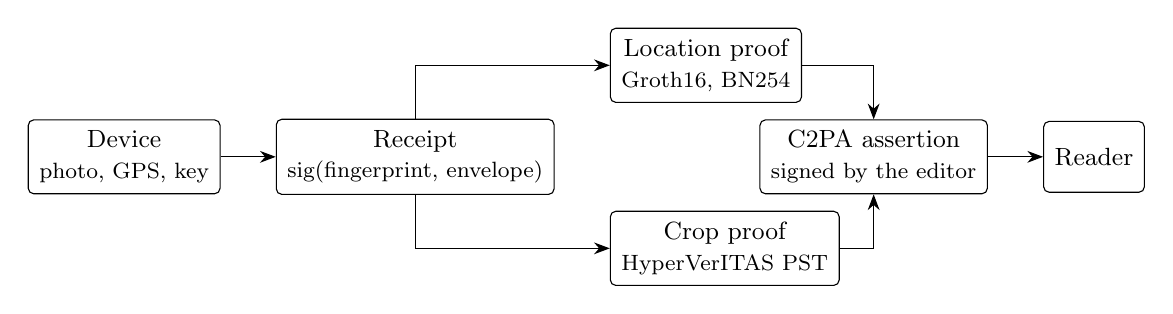
\begin{tikzpicture}[
  box/.style={draw,rounded corners=2pt,align=center,font=\small,minimum height=9mm,inner sep=4pt},
  arr/.style={-{Stealth[length=2mm]}},
  node distance=5mm and 7mm]
  \node[box] (dev) {Device\\\footnotesize photo, GPS, key};
  \node[box,right=of dev] (rec) {Receipt\\\footnotesize sig(fingerprint, envelope)};
  \node[box,above right=2mm and 7mm of rec] (loc) {Location proof\\\footnotesize Groth16, BN254};
  \node[box,below right=2mm and 7mm of rec] (crop) {Crop proof\\\footnotesize HyperVerITAS PST};
  \node[box,right=26mm of rec] (man) {C2PA assertion\\\footnotesize signed by the editor};
  \node[box,right=of man] (ver) {Reader};
  \draw[arr] (dev) -- (rec);
  \draw[arr] (rec) |- (loc);
  \draw[arr] (rec) |- (crop);
  \draw[arr] (loc) -| (man);
  \draw[arr] (crop) -| (man);
  \draw[arr] (man) -- (ver);
\end{tikzpicture}
\caption{The proof pipeline. The receipt is the only link between the two proofs.}
\end{figure}

A capture produces a $1024\times512$ RGB original $I$, a coordinate $(\theta,\phi)$
and a fresh salt $s$. The device signs a receipt over the fingerprint
$h_c = A\,I_c$ for each channel $c$ (a public $128\times2^{19}$ matrix $A$
over the BLS12-381 scalar field, as in VerITAS~\cite{veritas} \S4.2) and the
envelope $E=\mathrm{MiMC}(\theta,\phi,s)$. The location proof shows knowledge
of $(\theta,\phi,s)$ opening $E$ such that the coordinate maps to the published
H3 cell. The crop proof shows knowledge of $I$ with fingerprint $h$ whose left
half is the published image $P$; it commits to $I$ with the multilinear KZG
commitment of Papamanthou, Shi and Tamassia~\cite{pst} (PST). The reader runs four checks in order: the C2PA
manifest, the device signature over the receipt, the crop proof against
$(P,h)$, and the location proof against $(E,\text{cell})$.

We state the intended guarantees as four claims.
\begin{description}[itemsep=2pt]
  \item[C1, crop.] $P$ is the left half of the image the device fingerprinted.
  \item[C2, location.] The coordinate committed in the signed envelope lies in the published cell.
  \item[C3, binding.] Both proofs refer to the same capture, through the signed receipt.
  \item[C4, privacy.] The reader learns nothing about the original beyond $P$,
    and nothing about the coordinate beyond the cell.
\end{description}

The parties are the \emph{device}, which holds the signing key; the
\emph{photographer}, who holds the original and the secrets; the \emph{prover},
which may be the photographer or a newsroom backend; the \emph{reader}; and a
\emph{third party} who only has the published file.

\section{Summary}

\begin{table}[H]
\small
\begin{tabularx}{\textwidth}{@{}l X l l l@{}}
\toprule
ID & Finding & Breaks & Who & Status \\
\midrule
A1 & Trigonometric hints are not bound to the coordinate & C2 & prover & executed \\
A2 & Crop challenges do not depend on the published image & C1 & third party & executed \\
A3 & Range-check challenges are drawn before $H$ is committed & C1 & third party & executed \\
A4 & Commitments and fingerprint identify the original & C4 & reader & executed \\
A5 & Cell resolution is not bounded & C4 & photographer & executed \\
B1 & The device key attests whatever it signs & C1, C2 & device holder & executed \\
B2 & The editor signs with a public sample key & none & anyone & by inspection \\
B3 & Both setups are single-party & C1, C2 & setup operator & by inspection \\
\bottomrule
\end{tabularx}
\end{table}

\section{Soundness}

\begin{finding}{A1}{The trigonometric hints are not bound to the coordinate}
\item[What.] The circuit opens the envelope with the secret coordinate
  (\file{loc2index32/circuit.go}{36--37}) but computes the cell only from 16
  hint outputs per coordinate (\code{circuit.go}, lines 61 and 86). The hints are
  checked against each other (\file{circuit.go}{107--114}): $\gamma^2+\delta^2=1$,
  $\alpha\delta=\gamma$ and $2\gamma\delta=\beta$. No constraint relates them to
  $\theta$ or $\phi$; the only other uses of the coordinate are range checks
  (\file{circuit.go}{48--53}). ZKLP~\cite{zklp} \S4 argues soundness from these
  three identities: ``Soundness holds as $P_{ZKLP}$ evaluates that (i)
  $\gamma_\theta^2+\delta_\theta^2$ equals 1''. The values of any other angle
  satisfy them.
\item[Who.] Anyone who holds $(\theta,\phi,s)$: the photographer and any prover
  that receives the secrets. A third party cannot, because it must open $E$.
\item[Attack.] \code{TestAttackForgedHintsProveAnotherCell} in
  \code{location-proof/attack_test.go} keeps the honest envelope of a
  Buenos Aires coordinate, overrides the hint solver with the values for Tokyo
  Station, and proves with the unmodified circuit and proving key. The
  unmodified \code{verify} command accepts the proof for cell \code{872f5a32dffffff}
  (2.5\,s on an Apple M3 Pro). The honest CLI refuses to prove that cell, which
  shows that its native check is not a soundness boundary.
\item[Fix.] Two options. (a) The device computes the hints at capture and the
  envelope commits to them, $E=\mathrm{MiMC}(\theta,\phi,s,\text{hints})$, so
  the prover cannot change them. This is implemented on the fork's branch
  \code{c2p-77-sealed-hints} (\code{793d561}), not yet in the monorepo. We
  measured 21{,}161 to 23{,}793 constraints (+12.4\%). It moves trust: the cell
  is then correct for the hints the device signed, so the device is trusted for
  the trigonometry as well as for the coordinate. (b) Bound the hints in the
  circuit against a polynomial approximation of $\sin$ and $\cos$ of the
  coordinate. This keeps the trust model but costs more constraints; not
  measured.
\item[Status.] \status{executed}.
\end{finding}

\begin{finding}{A2}{The crop challenges do not depend on the published image}
\item[What.] The crop check is a Freivalds-style check: with one challenge $r_i$ per
  published pixel, the verifier checks $\sum_i r_i P_i = \sum_i r_i (S I)_i$ by
  sumcheck, where $S$ selects the left half. The challenges are drawn from a
  transcript that has absorbed only the image commitments, the hash sumchecks
  and the range-check messages (\file{crates/crop-proof/src/crop.rs}{238--285}).
  Neither $P$ nor $h$ is absorbed at any point; $P$ is read only after the
  challenges exist (\file{crop.rs}{309}). This is the weak Fiat--Shamir
  transformation of Bernhard, Pereira and Warinschi~\cite{weakfs}: the
  statement is not hashed. Trail of Bits reported the same class of bug in
  several proof systems as Frozen Heart~\cite{frozenheart}. The fingerprint enters only as the claimed sum of
  the hash sumcheck (\file{crop.rs}{248--251}). That gives no separate
  attack, because the device signs $h$ and a third party cannot choose it.
\item[Who.] A third party. The proof is public, so anyone can replay the
  transcript, obtain $r$, and look for $P'\neq P$ with
  $\sum_i r_i P'_i \equiv \sum_i r_i P_i \pmod p$ for each channel, with every
  $P'_i\in[0,255]$. The original is not needed. Republishing also needs a
  valid C2PA signature, which B2 makes free.
\item[Attack.] \code{fiat_shamir_substituted_crop_is_accepted} in
  \code{crates/crop-proof/tests/attack_fiat_shamir.rs}. From an honest proof
  of a random original, the test replays the verifier's transcript to obtain
  the $2^{18}$ challenges, starts from a smooth color gradient unrelated to
  the crop, and frees 64 pixels per channel. The gradient's claim misses the
  honest one by some $t$, so the free pixels must satisfy one congruence
  $\sum_{j} r_j\delta_j\equiv t \pmod p$ with small $\delta_j$. With 64
  unknowns and $p\approx2^{255}$ a solution of size about $p^{1/64}\approx2^4$
  exists. LLL reduction followed by Babai's nearest-plane algorithm finds it
  (\code{substitute_crop}
  in \code{crates/crop-proof/src/forge.rs}, with the solver in
  \code{src/lattice.rs}, pure Rust). The deltas stay within $\pm70$
  around mid-gray, so every pixel is in $[0,255]$. The forged image differs
  from the honest crop in 783{,}398 of 786{,}432 channel values and the
  unmodified verifier accepts it with the honest proof and fingerprint,
  unchanged. The whole test, including the honest proof it starts from, takes
  48\,s on an Apple M3 Pro.

  End to end, \code{substituted_crop_passes_every_reader_check} in
  \code{crates/provenance/tests/forged_crops.rs} applies the same substitution
  to the file \cmd{provenance demo} publishes. It keeps the receipt, the
  location proof and the crop proof, replaces the pixels with a color
  gradient, re-signs the manifest with the sample key (B2), and the reader
  passes all four checks.
\item[Fix.] Absorb the whole statement before the first challenge: a protocol
  and version tag, a digest of the verifier parameters, the crop rectangle, a
  digest of $P$, and $h$. Bump the proof format version so old proofs are
  rejected. VerITAS derives its hash challenge as $r\leftarrow H(A,h,pp,\mathrm{com}_v,\pi_{RP})$
  (\cite{veritas} \S5.4, Algorithm 3), so $h$ is part of the hashed statement there.
  A3's fix does not cover this one.
\item[Status.] \status{executed}.
\end{finding}

\begin{finding}{A3}{The range check draws its challenges before $H$ is committed}
\item[What.] HyperVerITAS needs every committed pixel in $[0,255]$, because the
  fingerprint is collision resistant only for low-norm preimages: ``To maintain
  soundness, we include a range proof'' (\cite{hyperveritas} \S1). The range
  proof is the HyperPlonk lookup~\cite{hyperplonk}: a product check between the
  pixels merged with the table $\{0,\dots,255\}$ and the sorted vector $H$, which
  lists the table and the pixel values together in table order. The challenges
  of that product check are drawn at \code{crates/crop-proof/src/iop.rs}, lines
  269 and 274, in the prover and at \file{crop.rs}{262--263} in the
  verifier, but the commitment to $H$ enters the transcript only after the crop
  sumcheck (\code{crop.rs}, lines 115 and 342).
\item[Who.] A third party. Choosing $H$ after the challenges lets the prover
  satisfy the product check for any committed values, in or out of range.
  Without the range bound, $A\,I'=h$ has solutions with arbitrary field
  entries: fix $I'$ to any chosen image on the left half and to anything on the
  right half, and solve a $128\times128$ linear system for 128 pixels of the
  right half. The forger needs only $h$, which is published in the receipt.
\item[Attack.] \code{forged_crop_of_another_picture_is_accepted} in
  \code{crates/crop-proof/tests/attack_range_check.rs}, with the dishonest
  prover in \code{crates/crop-proof/src/forge.rs} (built only with the
  \code{attack-hooks} feature). It signs nothing and never sees the original:
  from the fingerprint of a random original and a gray working image it proves
  that a color gradient is the left half of that original, and the unmodified
  verifier accepts. The lookup orders the positions of $H$ by powers of a
  generator $g$, and each nonzero entry enters two factors of the product: its
  own and that of the next position. The forged $H$ is zero except at two
  positions, so once the first value is fixed the second is the root of a
  quadratic; the first value changes when the discriminant is not a square. Prove and verify take 20\,s and 3.6\,GB on an
  Apple M3 Pro.

  End to end, \code{forged_crop_proof_passes_every_reader_check} in the same
  file as A2's takes the demo's published file, publishes a color gradient
  with a crop proof forged from the signed fingerprint, keeps the receipt and
  the location proof, re-signs the manifest with the sample key, and the
  reader passes all four checks. Both end-to-end tests take 38\,s together.
\item[Origin.] The reference implementation has the same order: in
  \code{hyperveritas_impl/examples/hv_crop_pst.rs} at \code{915c48a} the
  verifier draws the range challenges at lines 665--666 and absorbs the
  commitment to $H$ (\code{hCom}) at line 776. The other variants in that
  repository are listed in Section~\ref{sec:not-analyzed}.
\item[Fix.] Commit to $H$ and absorb the commitment before drawing the
  product-check challenges, as the HyperPlonk lookup requires. Check the same
  order for every committed polynomial. A2's fix does not cover this one: the
  attack works with the true statement.
\item[Status.] \status{executed}.
\end{finding}

\section{Privacy}

\begin{finding}{A4}{Commitments and fingerprint identify the original}
\item[What.] The fingerprint $h=A\,I$ is deterministic and public. The proof
  also carries PST commitments to the three channels of $I$
  (\file{crop.rs}{85--91}), and the commitment scheme adds no randomness
  (\file{multilinear_kzg/mod.rs}{102} in the HyperPlonk fork), so the same
  channel always gives the same commitment. Nine evaluations of the channel
  polynomials are published unmasked. HyperVerITAS derives zero knowledge from
  ``the hiding property of the commitments'' (\cite{hyperveritas}, proof of
  the linear hash protocol); our instantiation does not have it, so the gap is
  ours and not the paper's.
\item[Who.] Any reader with a candidate image. The candidate must match the
  original exactly as it was fingerprinted, after the resize to $1024\times512$. The device
  identifier also links every photo taken with one device.
\item[Attack.] \code{commitments_identify_the_original_image} in
  \code{crates/crop-proof/tests/attack_commitment_linkage.rs}. Committing to
  each channel of the true original under the public parameters reproduces the
  three commitments in the proof exactly, while flipping one bit of one pixel
  gives a different commitment. Recomputing the fingerprint from the original
  reproduces $h$. A reader can therefore confirm a guess of the full original,
  including the unpublished right half. The test takes 25\,s, almost all of it
  the honest proof.
\item[Fix.] A hiding commitment, zero-knowledge sumchecks and masked openings,
  plus a committed fingerprint that the device signs instead of $h$. This is a
  redesign; for this prototype we state that the proof is not zero knowledge
  with respect to the original.
\item[Status.] \status{executed}.
\end{finding}

\begin{finding}{A5}{The cell resolution is not bounded}
\item[What.] The verifier checks the location proof for whatever cell the
  assertion names. Nothing sets a coarsest allowed resolution, so the
  photographer chooses how much of the location to reveal.
\item[Attack.] \cmd{provenance attack} case \code{fine-cell} republishes the
  demo capture with a proof for its resolution-13 cell (about 44\,m$^2$); the
  verifier accepts.
\item[Observation.] At resolutions 14 and 15 the circuit's float32 mapping no
  longer matches H3 for our demo coordinate: the H3 grid coordinates the
  circuit computes are off by one or two units, so an honest prover cannot prove the true cell. We
  checked this natively, not in the circuit.
\item[Fix.] A resolution policy enforced by the verifier, and stated as the
  privacy parameter of the system.
\item[Status.] \status{executed}.
\end{finding}

\section{Trust boundary}

\begin{finding}{B1}{The device key attests whatever it signs}
\item[What.] The receipt is the only link between the photo and the location
  (C3). Whoever controls the key, or feeds the device a false coordinate,
  obtains a valid file for any photo and any place.
\item[Attack.] \cmd{provenance attack} case \code{signed-elsewhere} signs the
  demo photo with a Tokyo coordinate and proves that cell; the verifier
  accepts. In the CLI the simulated device key is an unencrypted PEM file
  protected only by file permissions (\file{crates/provenance/src/capture.rs}{233}).
  The same holds for the capture time: the receipt signs a \code{captured_at}
  that is ``asserted by the device, not by a trusted clock''
  (\file{capture.rs}{56}), and no claim in Section~2 covers time.
\item[Assumption.] The capture device is honest, reports its true location and
  time, and its key does not leave it. Hardware-backed keys and platform
  attestation would narrow this; they are not implemented.
\item[Status.] \status{executed}.
\end{finding}

\begin{finding}{B2}{The editor signs with a public sample key}
\item[What.] The C2PA manifest is signed with the sample certificate and key
  that \cmd{provenance setup} downloads from the public \code{c2patool}
  release, and the verifier accepts a manifest whose state is \code{Valid}
  (\file{crates/provenance/src/manifest.rs}{102--105}). Anyone can therefore
  re-sign a modified file. The check still verifies integrity, but it does not
  identify an editor. Every forged file in \cmd{provenance attack} is
  re-signed this way, so the rejections come from the receipt and the proofs.
\item[Status.] By inspection.
\end{finding}

\begin{finding}{B3}{Both setups are single-party}
\item[What.] \cmd{provenance setup} generates the Groth16 parameters and the
  KZG reference string locally. Whoever runs it could keep the trapdoors
  and forge either proof.
\item[Assumption.] The parameters come from an honest setup. A ceremony, or a
  transparent commitment scheme, would remove it.
\item[Status.] By inspection.
\end{finding}

\section{Assumptions outside the proof pipeline}\label{sec:assumptions}

These concern the phone web app and the capture server, which will change.
\begin{itemize}[itemsep=2pt]
  \item The server receives the exact coordinate, the salt and the original to
    build both proofs. We assume it is trusted with them.
  \item Phones pair with a six-digit code that does not expire and has no
    attempt limit; a paired key is added to the keys the reader trusts.
  \item The web app takes the photo from a file picker and reads the location
    when the file arrives, not at the shutter.
\end{itemize}

\section{Not analyzed}\label{sec:not-analyzed}

The following are part of the pipeline and were not examined. Nothing in this
document is a claim about them.
\begin{itemize}[itemsep=2pt]
  \item \textbf{Fingerprint parameters.} We did not check that 128 rows give
    collision resistance for $2^{19}$ pixels in $[0,255]$ over the BLS12-381
    scalar field, against the parameter analysis of VerITAS~\cite{veritas}.
  \item \textbf{Rounding near cell boundaries.} The circuit maps the
    coordinate to a cell with float32 arithmetic. Beyond the observation in
    A5, we did not check whether a coordinate near a cell boundary can be
    proven in a neighboring cell once A1 is fixed.
  \item \textbf{Displayed versus verified pixels.} The reader decodes the PNG
    and converts it to 8-bit RGB (\file{crates/provenance/src/capture.rs}{197--202}),
    dropping alpha and ignoring color profiles. We did not check whether a
    file can display a different picture from the one that is verified.
  \item \textbf{Other commitment schemes.} The HyperVerITAS repository has
    other variants of the crop proof; we checked only the transcript order of
    the PST variant we use (A3).
  \item \textbf{Libraries.} We rely on gnark's Groth16 verifier, the
    HyperPlonk polynomial commitment, \code{c2pa-rs} and the ECDSA
    implementation, and did not review them.
  \item \textbf{Denial of service.} Malformed inputs and resource use were not
    examined.
\end{itemize}

\section{Fix plan}

\begin{table}[H]
\small
\begin{tabularx}{\textwidth}{@{}l X X@{}}
\toprule
ID & Change & Test after the fix \\
\midrule
A1 & Seal the hints in the envelope (fork \code{793d561}) & forged hints fail to prove \\
A2 & Absorb the full statement before the first challenge & substituted crop rejected \\
A3 & Commit and absorb $H$ before the product-check challenges & forged range check rejected \\
A4 & Document; hiding is a redesign & unchanged \\
A5 & Resolution policy in the verifier & \code{fine-cell} rejected \\
B1--B3 & Documented assumptions & unchanged \\
\bottomrule
\end{tabularx}
\end{table}

\begin{thebibliography}{9}
\bibitem{zklp} J.~Ernstberger, C.~Zhang, L.~Ciprian, P.~Jovanovic, S.~Steinhorst.
  \emph{Zero-Knowledge Location Privacy via Accurate Floating-Point SNARKs}.
  IEEE S\&P 2025.
\bibitem{veritas} T.~Datta, B.~Chen, D.~Boneh.
  \emph{VerITAS: Verifying Image Transformations at Scale}. IEEE S\&P 2025.
\bibitem{hyperveritas} G.~Greiner, T.~Mowery, P.~Soni.
  \emph{HyperVerITAS: Verifying Image Transformations at Scale on Boolean
  Hypercubes}. Code: \url{https://github.com/C2PA-Thesis/HyperVerITAS}.
\bibitem{hyperplonk} B.~Chen, B.~B\"unz, D.~Boneh, Z.~Zhang.
  \emph{HyperPlonk: Plonk with Linear-Time Prover and High-Degree Custom Gates}.
  EUROCRYPT 2023.
\bibitem{pst} C.~Papamanthou, E.~Shi, R.~Tamassia.
  \emph{Signatures of Correct Computation}. TCC 2013.
\bibitem{weakfs} D.~Bernhard, O.~Pereira, B.~Warinschi.
  \emph{How Not to Prove Yourself: Pitfalls of the Fiat-Shamir Heuristic and
  Applications to Helios}. ASIACRYPT 2012.
\bibitem{frozenheart} Trail of Bits. \emph{Coordinated disclosure of
  vulnerabilities affecting Girault, Bulletproofs, and PlonK} (Frozen Heart), 2022.
\end{thebibliography}

\end{document}
